% Chapter Template

\chapter{Matériel et méthodes} % Main chapter title
\label{Materiel_methode} % Change X to a consecutive number; for referencing this chapter elsewhere, use \ref{ChapterX}

%----------------------------------------------------------------------------------------

\section{Support physique et numérique} %Spécificités ordinateur/machine virtuelle, python/libraries versions
L'ensemble des modélisations ont été réalisés sur une ordinateur portable hébergeant une machine virtuelle. Leurs caractéristiques sont rassemblées dans le tableau suivant :\\

\resizebox{18.75cm}{!}{
\begin{tabular}{| p{4cm} || l | l | p{5cm} | l | l |}
\hline
& Identifiant & Système d'explotation & Processeur & Mémoire vive & Carte graphique\\ \hline
Machine physique & ASUS ROG G75VW & Windows 7 64-bit SP1 & Intel Core I7-3610QM 2,30GHz (8CPU) &  
8 GB (DDR3) & NVIDIA GeForce GTX670M\\ \hline
Machine virtuelle (ressources allouées) & VirtualBox v.5.2.6 & Ubuntu 16.04 & 4 CPU, 90\% des ressources & 
5298 Mo & Support GPU non-utilisé\\ \hline
\end{tabular}
}

Les modélisation ont été réalisées à l'aide du language de programmation \href{https://www.python.org/}{Python} (version 3.6.4) renforcé de la librairie \href{https://www.tensorflow.org/}{TensorFlow} (version 1.4) et de l'interface graphique \href{https://jupyter.org/}{Jupyter}.\\
La base de données ayant servi à l'apprentissage et à l'évaluation du modèle correspond à la base de données \href{http://yann.lecun.com/exdb/mnist/}{MNIST}, contenant 70.000 images de chiffres manuscrits (60.000 pour l'entraînement, 10.000 pour l'évaluation), centrés et dont la taille a été normalisée. Chaque image est accompagnée d'un label décrivant quel chiffre elle contient.

%----------------------------------------------------------------------------------------

\section{Modèle POMDP} %Description du modèle perception-action, schéma explicatif
Le problème de recherche d'information dans un contexte d'exploraion de l'environnement visuel peut être formulé comme un \textbf{Processus de Décision Markovien Partiellement Observable} (POMDP ; \cite{Butko2010}). \\
Dans un POMDP, l'agent perçoit partiellement l'\textbf{état de l'environnement} à un temps \textit{t} -dans ce travail l'environnement visuel, perçut au travers d'un champs rétinien- et peut réaliser des \textbf{actions} -ici des saccades oculaires- qui peuvent avoir des conséquences l'environnement et sa perception. L'agent va ainsi construire un \textbf{état de croyance} -ici la catégorie prédite du stimulus- en fonction des observations et des actions réalisées jusqu'ici (\cite{Butko2010}).

\begin{figure}[th]
\centering
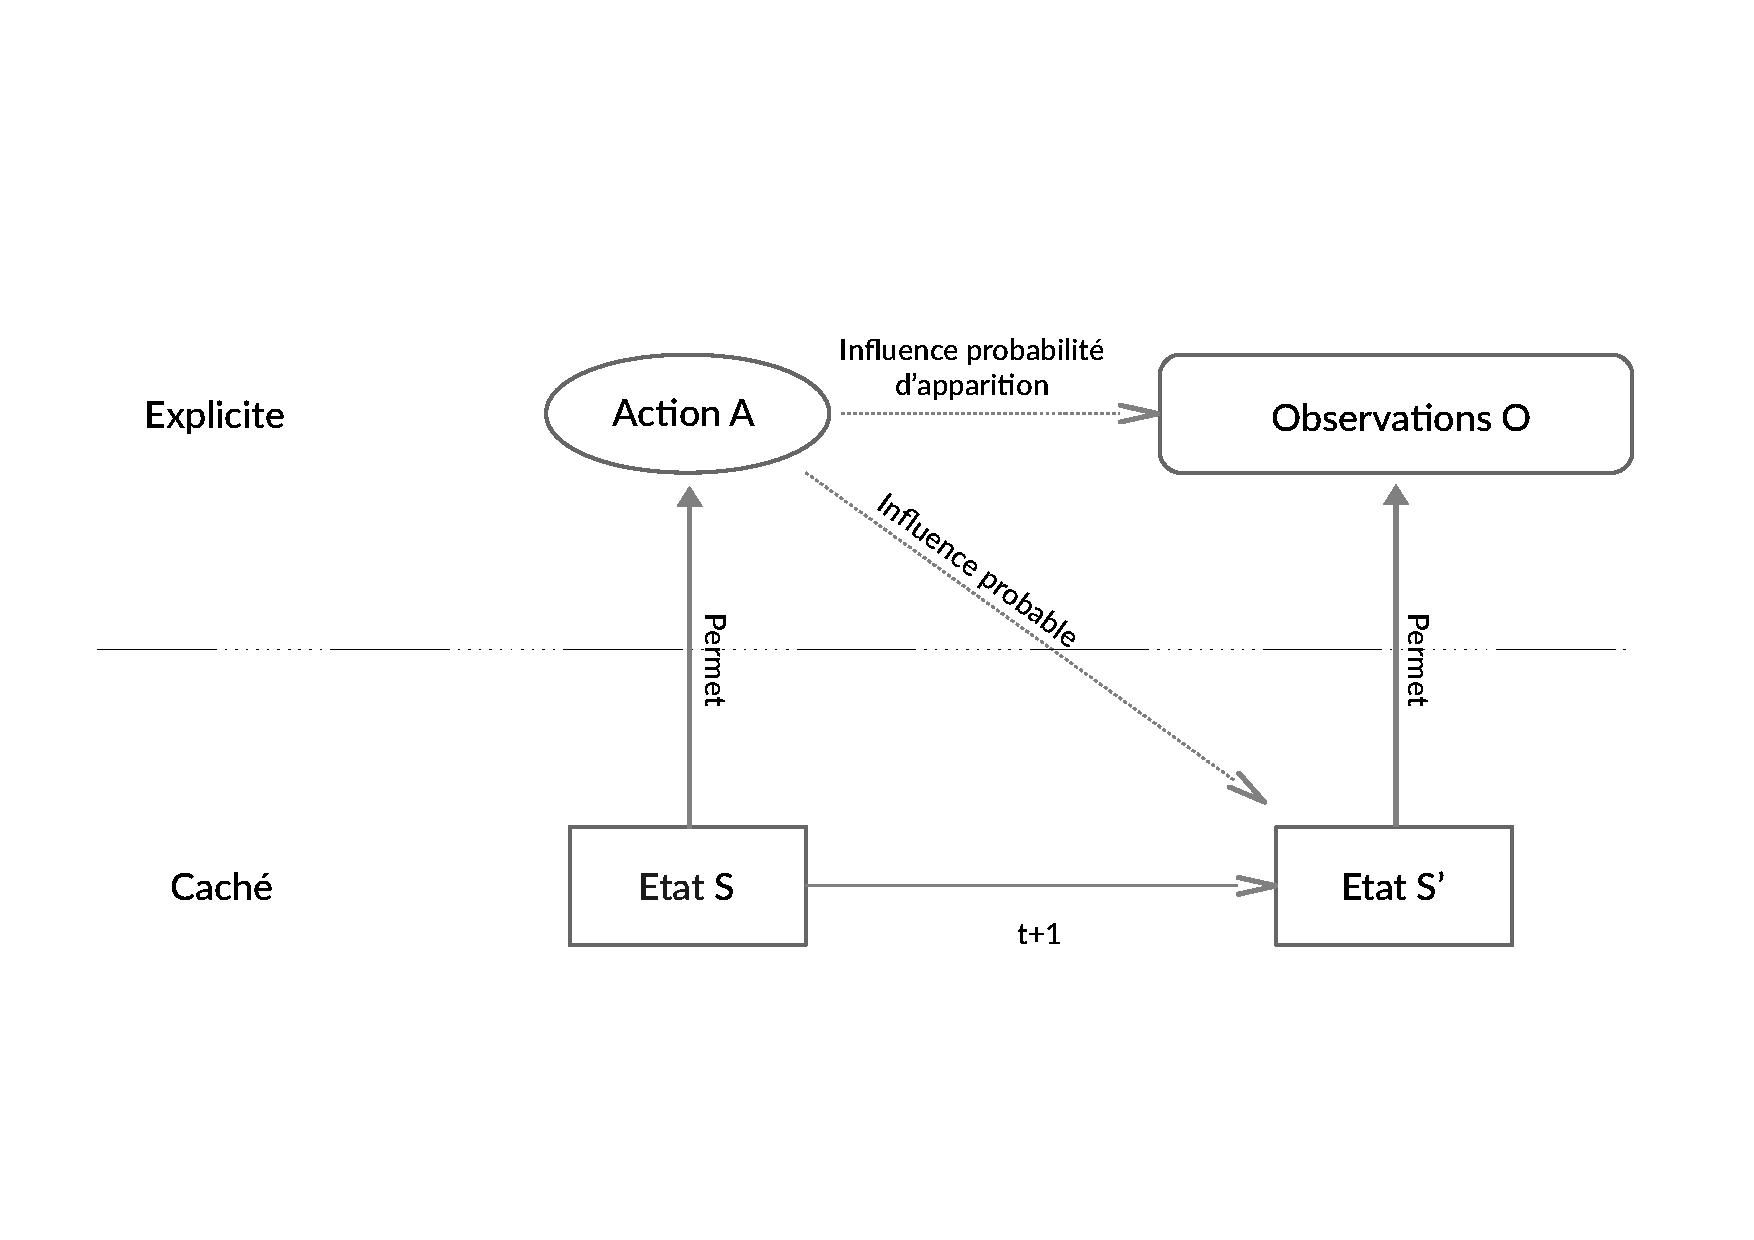
\includegraphics[scale=0.5]{Figures/POMDP}
\decoRule %puts an aesthetic horizontal line below the image
\caption[Figure]{Schéma des interations entre l'agent et son environnement au cours du temps dans un modèle POMDP}
\label{fig:POMDP}
\end{figure}

\begin{equation}
p(s_{t+1}|s_{1:t},a_{1:t},o_{1:t}) = p(s_{t+1}|s_{t},a_{t})
\label{eqn:POMDP_sta}
\end{equation}

\begin{equation}
p(o_{t}|s_{1:t},a_{1:t}) = p(o_{t}|s_{t},a_{t})
\label{eqn:POMDP_obs}
\end{equation}

\begin{equation}
B_{t}^i = p(S_{t} = i|A_{1:t},O_{1:t})
\label{eqn:POMDP_bel}
\end{equation}


%----------------------------------------------------------------------------------------

\section{Champs rétinien} %Description du modèle logpolar

%----------------------------------------------------------------------------------------

\section{Apprentissage supervisé} %Formules du modèle mathématiques soutenant la Régression linéaire multivariée
                                                                    %Prétraitements de l'image (whitening, resize et déplacement cible

\begin{equation}
h_{\theta}(x) = \theta^{T}x + b
\label{eqn:Hypo}
\end{equation}

\begin{equation}
J(\theta) = \frac{1}{2m} \sum_{i=1}^m (h_\theta(x^i)-y^i)^2
\label{eqn:Cost}
\end{equation}

\begin{equation}
\theta_j := \theta_j - \alpha \frac{1}{m} \sum_{i=1}^m (h_\theta(x^i) - y^i)x_{j}^i
\label{eqn:Grad_desc}
\end{equation}